\chapter{Testy i wyniki}
\label{cha5}

W tym rozdziale zostały przedstawione wszystkie wykonane badania wraz z ich wynikami. W badaniach zostały uwzględnione wszystkie metody uczenia maszynowego przedstawione w rozdziale \ref{cha:ucz.masz} rozszerzając podejścia przytoczone w przeglądzie literatury (rozdział \ref{cha:stan.badan}). Badania te stanowią uzupełnienie i rozszerzenie prac z \cite{Reczek21}. 

\section{Opis podejścia}
\label{opis_podejścia}
%  (czym się różni od tego z rozdz. 2)
W pierwszej kolejności wykorzystano momenty Hu w celu wyłuskania z obrazów cech, za pomocą których można byłoby przeprowadzić klasyfikację. Analogicznie przetestowano tekstury Haralicka. Następnie liczby te podawano na wejście klasycznych klasyfikatorów. Kolejne testy objęły uogólnioną transformatę Hougha. Po zakończeniu tych testów rozpoczęto badania nad bardziej skomplikowanymi metodami. Przede wszystkim zdecydowano, aby rozpoznawać jakość zdjęć na podstawie liczby struktur różnych klas na obrazach. Szczegóły dotyczące wycinania, tworzenia bazy danych i rozpoznawania tych struktur zostały przedstawione w rozdziale \ref{}. W tym celu wykorzystano również wszystkie klasyfikatory klasyczne przedstawione w rozdziale \ref{cha:Wykorzystane metody uczenia maszynowego}. Wyniki porównano uwzględniając wiele aspektów, jak interpretowalność wyników, łatwość implementacji, prostotę algorytmu czy czas uczenia. Aby mieć ogląd całej sytuacji przetestowano również najskuteczniejsze obecnie architektury sieci neuronowych wykorzystywanych w celach klasyfikacji obrazów i również zostały one porównane wielopłaszczyznowo z pozostałymi wynikami. 

% ############ Klasyfikacja struktur i ocena jakości odlewów #############
\section{Klasyfikacja struktur i ocena jakości odlewów}
\label{sec:klasyfikacja_struktur}

Jest to najszerszy obszar badań, ponieważ dzięki danym w postaci zliczonych struktur można sprawdzić, czy kształty tych struktur mają wpływ na właściwości mechaniczne odlewów, a jeśli tak, to w jakim stopniu. Jak wszyscy wiemy, sieci neuronowe, które odbierają obrazy w postaci pikseli jako dane wejściowe i zwracają wynik w postaci „tak” lub „nie” na pytanie, czy wytrzymałość na rozciąganie danej mikrostruktury jest duża (lub mała) są modelami „czarnej skrzynki”, co oznacza, że trudno zweryfikować, dlaczego model podjął jedną decyzję nad drugą. Wykorzystując jednak dane w postaci liczby struktur i ich klas, można pokusić się o zbudowanie interpretowalnego modelu.

% ############ Klasyfikacja struktur i ocena jakości odlewów #############
\subsection{Momenty Hu oraz tekstury Haralicka}
\label{sec:hu_haralick}

Pierwszym podejściem było wykorzystanie tekstur Haralicka i momentów Hu do zidentyfikowania struktur na zdjęciu. Implementacja metody momentów Hu została zaczerpnięta z pakietu \ita{opencv-python}, natomiast implementacja tekstur Haralicka została zaczerpnięta z modułu \ita{mahotas}. Może się wydawać, że użycie tych algorytmów jest poprawne i przyniesie pożądane rezultaty, ponieważ zostały zaprojektowane specjalnie do tego celu. Rysunek \ref{fig:mesh20} przedstawia dwa zdjęcia różnych mikrostruktur, które potencjalnie można zidentyfikować przy użyciu technik opisanych powyżej.
\begin{figure}[h]
	\centering
	\begin{subfigure}{0.47\textwidth}
	    \centering
	    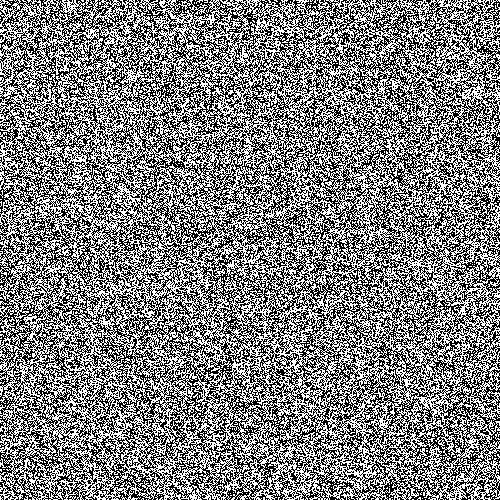
\includegraphics[width=1\textwidth]{rys.20.przyklad.mikrostruktur.a.png}
	    \subcaption{\label{subfigure_a}Zdjęcie mikrostruktury z obiektami klasy I}
	\end{subfigure}
	\begin{subfigure}{0.47\textwidth}
	    \centering
	    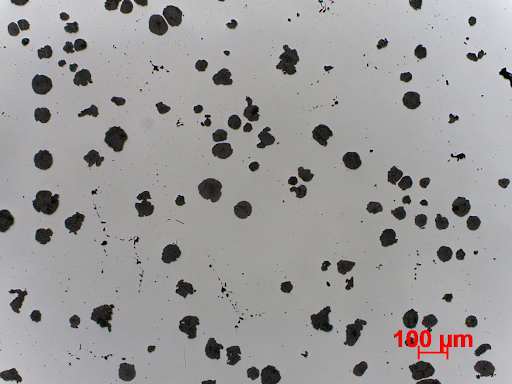
\includegraphics[width=1\textwidth]{rys.20.przyklad.mikrostruktur.b.png}
	    \subcaption{\label{subfigure_b}Zdjęcie mikrostruktury z obiektami klasy V}
	\end{subfigure}
	\caption{\label{fig:mesh20}Dwa przykładowe zdjęcia mikrostruktur. Ich tekstury i znajdujące się tam kształty diametralnie się różnią. Źródło: \cite{Pirowski17}}
\end{figure}
W pierwszym eksperymencie wykorzystano tekstury Haralicka, momenty Hu i model maszyny wektorów nośnych (SVM). Niestety taka konfiguracja modeli nie przyniosła oczekiwanych rezultatów. Testy przeprowadzono z wykorzystaniem sprawdzianu krzyżowego (ang. \ita{cross-validation}), a dokładnie sprawdzian k-krotny, w którym oryginalna próba jest dzielona na \ita{k} podzbiorów, po czym każdy z tych podzbiorów jest wykorzystywany jako zbiór testowy, gdzie w tym czasie wszystkie pozostałe są wykorzystywane jako zbiór trenignowy. Następnie te \ita{k} rezultatów jest uśrednianych. Otrzymane w ten sposób wyniki wyniosły zaledwie 55\%. W rezultacie, skoro najprostsze podejścia zawodzą, zdecydowano się na nieco bardziej złożoną strategię.

\subsection{Uogólniona transformata Hougha}
\label{hough}



% chyba bym się w sumie nie trzymał tego schematu, tylko chronologicznie i jednoczesnie Rm i Rp ;d
%5.2. Opis wykonanych badań i testów oraz własnej implementacji
%
%5.3. Omówienie wyników uzyskanych za pomocą metod klasycznych
%
%5.3.1. Analiza wytrzymałości na rozciąganie
%
%5.3.2. Analiza granicy plastyczności
%
%5.4. Omówienie wyników uzyskanych za pomocą sieci neuronowych
%
%5.4.1. Analiza wytrzymałości na rozciąganie
%
%5.4.2. Analiza granicy plastyczności
%
%5.5. Omówienie wyników / całościowe
